\documentclass[../main.tex]{subfiles}

\begin{document}
\chapter*{Numerical Integration of Functions}

\begin{center}\begin{Large}\textbf{CHAPTER OBJECTIVES}\end{Large}\end{center}

The primary objective of this chapter is to introduce you to numerical methods for
integrating given functions. Specific objectives and topics covered are
\begin{itemize}
\item Understanding how Richardson extrapolation provides a means to create a more
accurate integral estimate by combining two less accurate estimates.
\item Understanding how Gauss quadrature provides superior integral estimates by
picking optimal abscissas at which to evaluate the function.
\item Knowing how to use MATLAB's built-in functions $quad$ and 
$quadl$ to integrate
functions.
\end{itemize}
\vspace{0,6in}
\section{INTRODUCTION}
\vspace{0,1in}
\hrule
\vspace{0,1in}
In Chap. 19, we noted that functions to be integrated numerically will typically be of two
forms: a table of values or a function. The form of the data has an important influence on
the approaches that can be used to evaluate the integral. For tabulated information, you are
limited by the number of points that are given. In contrast, if the function is available, you
can generate as many values of $f (x)$ as are required to attain acceptable accuracy

At face value, the composite Simpson's 1/3 rule might seem to be a reasonable tool for
such problems. Although it is certainly adequate for many problems, there are more efficient methods that are available. This section is devoted to three such techniques, which
capitalize on the ability to generate function values to develop efficient schemes for
numerical integration.

The first technique is based on Richardson extrapolation, which is a method for
combining two numerical integral estimates to obtain a third, more accurate value. The
computational algorithm for implementing Richardson extrapolation in a highly efficient
manner is called Romberg integration. This technique can be used to generate an integral
estimate within a prespecified error tolerance.

The second method is called Gauss quadrature. Recall that, in Chap. 19, values of
$f (x)$ for the Newton-Cotes formulas were determined at specified values of $x$. For example, if we used the trapezoidal rule to determine an integral, we were constrained to take the
weighted average of $f (x)$ at the ends of the interval. Gauss-quadrature formulas employ $x$
values that are positioned between the integration limits in such a manner that a much more
accurpartate integral estimate results.

The third approach is called $adaptive\, quadrature$. This techniques applies composite
Simpson s 1/3 rule to subintervals of the integration range in a way that allows error estimates to be computed. These error estimates are then used to determine whether more
refined estimates are required for a subinterval. In this way, more refined segmentation
is only used where it is necessary. Two built-in MATLAB functions that use adaptive quadrature are illustrated.


\vspace{0,6in}
\section{ROMBERG INTEGRATION}
\vspace{0,1in}
\hrule
\vspace{0,1in}
Romberg integration is one technique that is designed to attain efficient numerical integrals
of functions. It is quite similar to the techniques discussed in Chap. 19 in the sense that it
is based on successive application of the trapezoidal rule. However, through mathematical
manipulations, superior results are attained for less effort.


\subsection{Richardson Extrapolation}
Techniques are available to improve the results of numerical integration on the basis of the
integral estimates themselves. Generally called $Richardson\, extrapolation$, these methods
use two estimates of an integral to compute a third, more accurate approximation.


The estimate and the error associated with the composite trapezoidal rule can be represented generally as

	\begin{flushleft}
	$I=I(h)+E(h)$
	\end{flushleft}
	
where $I$ = the exact value of the integral, $I(h)$ = the approximation from an n-segment
application of the trapezoidal rule with step size $h = (b − a)/n$, and $E(h)$ = the truncation
error. If we make two separate estimates using step sizes of $h_1$ and $h_2$ and have exact values for the error:\\
\begin{equation}
	\tag{20.1}
	I(h_1)+E(h_1)=I(h_2)+E(h_2)
\end{equation}\\
Now recall that the error of the composite trapezoidal rule can be represented approximately by Eq. (19.21) [with $n = (b − a)/h$]:
\begin{equation}
	\tag{20.2}
	E\cong-\dfrac{b-a}{12}h^{2}\bar{f}''
\end{equation}
If it is assumed that $\bar{f}$ is constant regardless of step size, Eq. (20.2) can be used to determine that the ratio of the two errors will be
\begin{equation}
	\tag{20.3}
	\dfrac{E(h_1)}{E(h_2)}\cong\dfrac{h^{2}_{1}}{h^{2}_{2}}
\end{equation}\\
This calculation has the important effect of removing the term $\bar{f}$ from the computation.
In so doing, we have made it possible to utilize the information embodied by Eq. (20.2) without prior knowledge of the function's second derivative. To do this, we rearrange
Eq. (20.3) to give

	$$E(h_1) \cong E(h_2)\left(\dfrac{h_1}{h_2} \right)^2$$\\
which can be substituted into Eq. (20.1):

	$$I(h1)+E(h_2)\left(\dfrac{h_1}{h_2} \right)^2=I(h_2)+E(h_2)$$\\
which can be solved for

	$$E(h_2)=\dfrac{(I(h_1)-I(h_2)}{1-(h_1/h_2)^2}$$\\
Thus, we have developed an estimate of the truncation error in terms of the integral estimates and their step sizes. This estimate can then be substituted into

	$$I=I(h_2)+E(h_2)$$\\
to yield an improved estimate of the integral:
\begin{equation}
	\tag{20.4}
	I=I(h_2)+\dfrac{1}{(h_1/h_2)^2-1}[I(h_2)-I(h_1)]
\end{equation}

It can be shown (Ralston and Rabinowitz, 1978) that the error of this estimate is
$O(h^4)$. Thus, we have combined two trapezoidal rule estimates of $O(h^2)$ to yield a new estimate of $O(h^4)$. For the special case where the interval is halved $(h_2 = h_1/2)$, this equation becomes
\begin{equation}
	\tag{20.5}
	I=\dfrac{4}{3}I(h_2)-\dfrac{1}{3}I(h_1)
\end{equation}

\subsection{Richardson Extrapolation}
\textbf{Problem Statement.} Use Richardson extrapolation to evaluate the integral of $f(x) =
0.2 + 25x − 200x^2 + 675x^3 − 900x^4 + 400x^5$ from $a = 0$ to $b = 0.8.$\\
\vspace{0.1in}
\textbf{Solution.} Single and composite applications of the trapezoidal rule can be used to evaluate the integral:\\


\begin{tabular}{cccc}
	\hline
	\textbf{Segments} & \textbf{$h$} & \textbf{Integral} & \textbf{$\varepsilon_t$}\\ \hline
	1 & 0,8 & 0,1728 & 89.5\%\\
	2 & 0.4 & 1.0688 & 34.9\%\\
	4 & 0.2 & 1.4848 & 9.5\%\\ \hline
\end{tabular}\\

\vspace{0.5in}
Richardson extrapolation can be used to combine these results to obtain improved estimates
of the integral. For example, the estimates for one and two segments can be combined to yield
	
	$$I=\dfrac{4}{3}(1.0688)-\dfrac{1}{3}(0.1728)=1.367467$$\\
The error of the improved integral is $E_t = 1.640533 − 1.367467 = 0.273067(\varepsilon_t = 16.6\%)$, 
which is superior to the estimates upon which it was based.

In the same manner, the estimates for two and four segments can be combined to give

	$$I=\dfrac{4}{3}(1.4848)-\dfrac{1}{3}(1.0688)=1.623467$$\\
which represents an error of $E_t = 1.640533 − 1.623467 = 0.017067 (\varepsilon_t = 1.0\%)$.

\vspace{0.3in}
Equation (20.4) provides a way to combine two applications of the trapezoidal rule
with error $O(h^2)$ to compute a third estimate with error $O(h^4)$. This approach is a subset of
a more general method for combining integrals to obtain improved estimates. For instance,
in Example 20.1, we computed two improved integrals of $O(h^4)$ on the basis of three trapezoidal rule estimates. These two improved integrals can, in turn, be combined to yield an
even better value with $O(h^6)$. For the special case where the original trapezoidal estimates
are based on successive halving of the step size, the equation used for $O(h^6)$ accuracy is
\begin{equation}
	\tag{20.6}
	I=\dfrac{16}{15}I_m-\dfrac{1}{15}I_l
\end{equation}\\
where $I_m$ and $I_l$ are the more and less accurate estimates, respectively. Similarly, two
$O(h^6)$ results can be combined to compute an integral that is $O(h^8)$ using
\begin{equation}
	\tag{20.7}
	I=\dfrac{64}{63}I_m-\dfrac{1}{63}I_l
\end{equation}


\subsection{Higher-Order Corrections}
\textbf{Problem Statement.}  In Example 20.1, we used Richardson extrapolation to compute two
integral estimates of $O(h^4)$. Utilize Eq. (20.6) to combine these estimates to compute an
integral with $O(h^6)$.\\

\textbf{Solution.} The two integral estimates of $O(h^4)$ obtained in Example 20.1 were 1.367467
and 1.623467. These values can be substituted into Eq. (20.6) to yield

	$$I=\dfrac{16}{15}(1.623467)-\dfrac{1}{15}(1.367467)=1.640533$$\\
which is the exact value of the integral.

\subsection{ The Romberg Integration Algorithm}
Notice that the coefficients in each of the extrapolation equations [Eqs. (20.5), (20.6), and
(20.7)] add up to 1. Thus, they represent weighting factors that, as accuracy increases,place relatively greater weight on the superior integral estimate. These formulations can be
expressed in a general form that is well suited for computer implementation:
\begin{equation}
	\tag{20.8}
	I_{j,k}=\dfrac{4^{k-1}I_{j+1,k-1}-I_{j,k-1}}{4^{k-1}-1}
\end{equation}
where $I_{j+1,k−1}$ and $I_{j,k−1}$ = the more and less accurate integrals, respectively, and $I_{j,k}$ =
the improved integral. The index $k$ signifies the level of the integration, where $k$ = 1 corresponds to the original trapezoidal rule estimates, k = 2 corresponds to the $O(h^4)$ estimates, $k$ = 3 to the $O(h^6)$, and so forth. The index $j$ is used to distinguish between the more
$(j + 1)$ and the less $(j)$ accurate estimates. For example, for $k$ = 2 and $j$ = 1, Eq. (20.8)
becomes
\begin{equation}
	I_{1,2}=\dfrac{4I_{2,1}-I_{1,1}}{3}
\end{equation}
which is equivalent to Eq. (20.5).
\vspace{0.5 in}

The general form represented by Eq. (20.8) is attributed to Romberg, and its systematic application to evaluate integrals is known as Romberg integration. Figure 20.1 is a
graphical depiction of the sequence of integral estimates generated using this approach.
Each matrix corresponds to a single iteration. The first column contains the trapezoidal rule
evaluations that are designated $I_{j,1}$, where $j$ = 1 is for a single-segment application (step
size is $b − a$), $j$ = 2 is for a two-segment application [step size is ($b − a)/2$], $j$ = 3 is for
a four-segment application [step size is ($b − a)/4$], and so forth. The other columns of the
matrix are generated by systematically applying Eq. (20.8) to obtain successively better
estimates of the integral.

r example, the first iteration (Fig. 20.1a) involves computing the one- and twosegment trapezoidal rule estimates ($I_{1,1}$ and $I_{2,1}$). Equation (20.8) is then used to compute
the element $I_{1,2 = 1.367467}$, which has an error of $O(h^4)$.


\begin{figure}[hbt!]
	\centering
	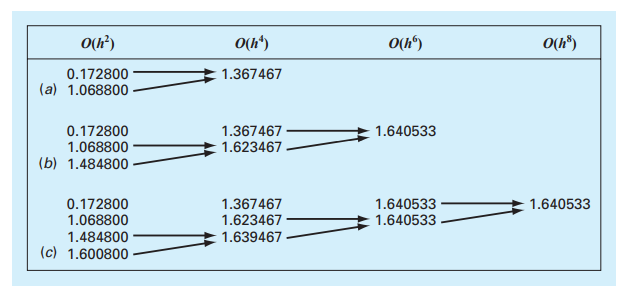
\includegraphics[width=0.75\textwidth]{pic_20_1}
	\caption{\textsf{Graphical depiction of the sequence of integral estimates generated using Romberg integration.
(a) First iteration. (b) Second iteration. (c) Third iteration.}} \hrule
	\label{pic.20.1}
\end{figure}
\vspace{0.3in}

Now, we must check to determine whether this result is adequate for our needs. As in
other approximate methods in this book, a termination, or stopping, criterion is required to
assess the accuracy of the results. One method that can be employed for the present purposes is
\begin{equation}
	\tag{20.9}
	|\varepsilon_a|=\left|\dfrac{I_{1,k}-I_{2,k-1}}{I_{1,k}} \right| x100\%
\end{equation}\\
where $\varepsilon_a$ = an estimate of the percent relative error. Thus, as was done previously in other
iterative processes, we compare the new estimate with a previous value. For Eq. (20.9), the
previous value is the most accurate estimate from the previous level of integration (i.e., the
$k − 1$ level of integration with $j = 2$). When the change between the old and new values
as represented by εa is below a prespecified error criterion εs, the computation is terminated. For Fig. 20.1a, this evaluation indicates the following percent change over the
course of the first iteration:

	$$|\varepsilon_a|= \left|\dfrac{1.367467 − 1.068800}{1.367467} \right| \: x \: 100\% = 21.8\%$$
	
The object of the second iteration (Fig. 20.1b) is to obtain the $O(h^6)$ estimate—$I_{1,3}$.
To do this, a four-segment trapezoidal rule estimate, $I_{3,1} = 1.4848$, is determined. Then it
is combined with $I_{2,1}$ using Eq. (20.8) to generate $I_{2,2} = 1.623467$. The result is, in turn,
combined with $I_{1,2}$ to yield $I_{1,3} = 1.640533$. Equation (20.9) can be applied to determine
that this result represents a change of $1.0\%$ when compared with the previous result $I_{2,2}$.

The third iteration (Fig. 20.1c) continues the process in the same fashion. In this case,
an eight-segment trapezoidal estimate is added to the first column, and then Eq. (20.8) is
applied to compute successively more accurate integrals along the lower diagonal. After
only three iterations, because we are evaluating a fifth-order polynomial, the result
$(I_{1,4} = 1.640533)$ is exact.

Romberg integration is more efficient than the trapezoidal rule and Simpson's rules.
For example, for determination of the integral as shown in Fig. 20.1, Simpson's 1/3 rule
would require about a 48-segment application in double precision to yield an estimate of
the integral to seven significant digits: 1.640533. In contrast, Romberg integration produces the same result based on combining one-, two-, four-, and eight-segment trapezoidal
rules—that is, with only 15 function evaluations!

Figure 20.2 presents an M-file for Romberg integration. By using loops, this algorithm
implements the method in an efficient manner. Note that the function uses another function
trap to implement the composite trapezoidal rule evaluations (recall Fig. 19.10). Here is
a MATLAB session showing how it can be used to determine the integral of the polynomial
from Example 20.1:

\begin{verbatim}
>> f=@(x) 0.2+25*x-200*x^2+675*x^3-900*x^4+400*x^5;
>> romberg(f,0,0.8)

ans =
    1.6405
\end{verbatim}

\begin{figure}[hbt!]
	\centering
	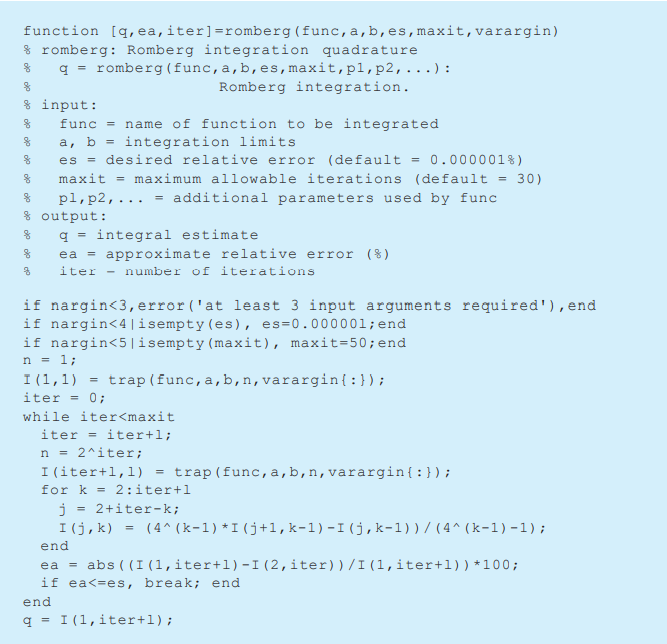
\includegraphics[width=0.75\textwidth]{pic_20_2}
	\caption{\textsf{M-file to implement Romberg integration.}} \hrule
	\label{pic.20.2}
\end{figure}

\vspace{0,3in}
\section{GAUSS QUADRATURE}
\vspace{0,1in}
\hrule
\vspace{0,1in}
In Chap. 19, we employed the Newton-Cotes equations. A characteristic of these formulas
(with the exception of the special case of unequally spaced data) was that the integral estimate was based on evenly spaced function values. Consequently, the location of the base
points used in these equations was predetermined or fixed.

For example, as depicted in Fig. 20.3$a$, the trapezoidal rule is based on taking the area
under the straight line connecting the function values at the ends of the integration interval.
The formula that is used to compute this area is
\begin{equation}
	\tag{20.10}
	I\cong (b-a)\dfrac{f(a)+f(b)}{2}
\end{equation}
\pagebreak
\begin{figure}[hbt!]
	\centering
	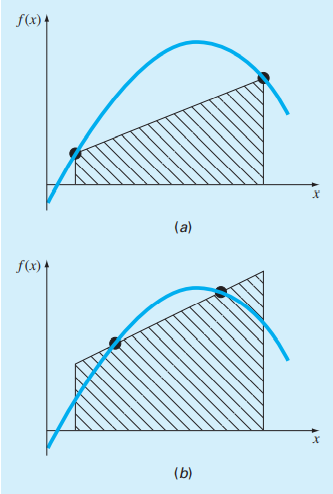
\includegraphics[width=0.55\textwidth]{pic_20_3}
	\caption{\textsf{(a) Graphical depiction of the trapezoidal rule as the area under the straight line joining fixed
end points. (b) An improved integral estimate obtained by taking the area under the straight line
passing through two intermediate points. By positioning these points wisely, the positive and 
negative errors are better balanced, and an improved integral estimate results.}} \hrule
	\label{pic.20.3}
\end{figure}\\
\vspace{0.1in}\\
where $a$ and $b$ = the limits of integration and $b − a$ = the width of the integration interval.
Because the trapezoidal rule must pass through the end points, there are cases such as
Fig. 20.3$a$ where the formula results in a large error.

Now, suppose that the constraint of fixed base points was removed and we were free to
evaluate the area under a straight line joining any two points on the curve. By positioning
these points wisely, we could define a straight line that would balance the positive and negative errors. Hence, as in Fig. 20.3$b$, we would arrive at an improved estimate of the integral.

$Gauss\, quadrature$ is the name for a class of techniques to implement such a strategy.
The particular Gauss quadrature formulas described in this section are called $GaussLegendre$ formulas. Before describing the approach, we will show how numerical integration formulas such as the trapezoidal rule can be derived using the method of undetermined
coefficients. This method will then be employed to develop the Gauss-Legendre formulas.


\subsection{Method of Undetermined Coefficients}
In Chap. 19, we derived the trapezoidal rule by integrating a linear interpolating polynomial
and by geometrical reasoning. The method of undetermined coefficients offers a third approach that also has utility in deriving other integration techniques such as Gauss quadrature.\\
\begin{figure}[hbt!]
	\centering
	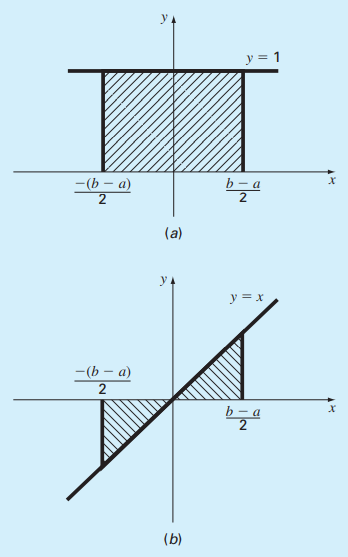
\includegraphics[width=0.55\textwidth]{pic_20_4}
	\caption{\textsf{Two integrals that should be evaluated exactly by the trapezoidal rule: (a) a constant and 
(b) a straight line.}} \hrule
	\label{pic.20.4}
\end{figure}

To illustrate the approach, Eq. (20.10) is expressed as
\begin{equation}
	\tag{20.11}
	I\cong c_0 f(a) + c_1 f(b)
\end{equation}\\
where the $c's$ = constants. Now realize that the trapezoidal rule should yield exact results
when the function being integrated is a constant or a straight line. Two simple equations
that represent these cases are $y = 1$ and $y = x$ (Fig. 20.4). Thus, the following equalities
should hold:

	$$c_0 + c_1 = \int^{(b-a)/2}_{-(b-a)/2} 1dx$$\\
and

	$$-c_0 \dfrac{b-a}{2}+c_1 \dfrac{b-a}{2} = \int^{(b-a)/2}_{-(b-a)/2} x\, dx$$\\
or, evaluating the integrals,

	$$c_0 + c_1 = b-a$$\\
and

	$$-c_0 \dfrac{b-a}{2} + c_1 \dfrac{b-a}{2} = 0$$
These are two equations with two unknowns that can be solved for

	$$c_0= c_1 = \dfrac{b-a}{2}$$
which, when substituted back into Eq. (20.11), gives

	$I= \dfrac{b-a}{2} f(a) + \dfrac{b-a}{2} f(b)$
which is equivalent to the trapezoidal rule.
\subsection{Derivation of the Two-Point Gauss-Legendre Formula}
Just as was the case for the previous derivation of the trapezoidal rule, the object of Gauss
quadrature is to determine the coefficients of an equation of the form
\vspace{0.1 in}
\begin{equation}
	\tag{20.12}
	I\cong c_0 f(x_0)+c_1 f(x_1)
\end{equation}
where the $c's$ = the unknown coefficients. However, in contrast to the trapezoidal rule that
used fixed end points $a$ and $b$, the function arguments $x_0$ and $x_1$ are not fixed at the end
points, but are unknowns (Fig. 20.5). Thus, we now have a total of four unknowns that
must be evaluated, and consequently, we require four conditions to determine them exactly.

Just as for the trapezoidal rule, we can obtain two of these conditions by assuming
that Eq. (20.12) fits the integral of a constant and a linear function exactly. Then, to arrive at
the other two conditions, we merely extend this reasoning by assuming that it also fits the
integral of a parabolic $(y = x^2)$ and a cubic $(y = x^3)$ function. By doing this, we determine
\pagebreak
\begin{figure}[hbt!]
	\centering
	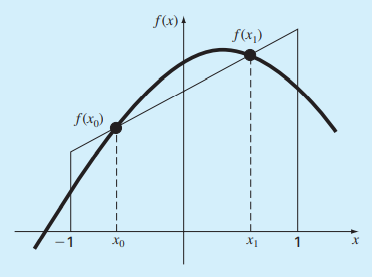
\includegraphics[width=0.55\textwidth]{pic_20_5}
	\caption{\textsf{Graphical depiction of the unknown variables x0 and x1 for integration by Gauss quadrature.}} \hrule
	\label{pic.20.5}
\end{figure}\\
all four unknowns and in the bargain derive a linear two-point integration formula that is
exact for cubics. The four equations to be solved are
\begin{equation}
	\tag{20.13}
	c_0+c_1 = \int^{1}_{-1} 1dx = 2
\end{equation}
\begin{equation}
	\tag{20.14}
	c_0 x_0 + c_1 x_1 = \int^{1}_{-1} xdx = 0
\end{equation}
\begin{equation}
	\tag{20.15}
	c_0 x^{2}_{0} + c_1 x^{2}_{1} = \int^{1}_{-1} x^2 dx = \dfrac{2}{3}
\end{equation}
\begin{equation}
	\tag{20.16}
	c_0 x^{3}_{0} + c_1 x^{3}_{1} = \int^{1}_{-1} x^3 \, dx = 0
\end{equation}

Equations (20.13) through (20.16) can be solved simultaneously for the four unknowns.
First, solve Eq. (20.14) for c1 and substitute the result into Eq. (20.16), which can be solved for

	$$x^{2}_{0} = x^{2}_{1}$$\\
Since $x_0$ and $x_1$ cannot be equal, this means that $x_0 = −x_1$. Substituting this result into
Eq. (20.14) yields $c_0 = c_1$. Consequently from Eq. (20.13) it follows that

	$$c_0 = c_1 = 1$$\\
Substituting these results into Eq. (20.15) gives

	$$x_0 = -\dfrac{1}{\sqrt{3}} = −0.5773503 ...$$
	
	$$x_1 = \dfrac{1}{\sqrt{3}} = 0.5773503 ...$$\\
Therefore, the two-point Gauss-Legendre formula is

\begin{equation}
	\tag{20.17}
	I=f \left(\dfrac{-1}{\sqrt{3}} \right) + f \left(\dfrac{1}{\sqrt{3}} \right)
\end{equation}\\
Thus, we arrive at the interesting result that the simple addition of the function values at $x = −1/\sqrt{3}$ and $1/\sqrt{3}$ yields an integral estimate that is third-order accurate.

Notice that the integration limits in Eqs. (20.13) through (20.16) are from $-1$ to $1$. This
was done to simplify the mathematics and to make the formulation as general as possible.
A simple change of variable can be used to translate other limits of integration into this
form. This is accomplished by assuming that a new variable xd is related to the original
variable x in a linear fashion, as in
\begin{equation}
	\tag{20.18}
	x = a_1 + a_2x_d
\end{equation}\\
If the lower limit, $x = a$, corresponds to $x_d = −1$, these values can be substituted into
Eq. (20.18) to yield
\begin{equation}
	\tag{20.19}
	a=a_1 + a_2(-1)
\end{equation}\\
Similarly, the upper limit, $x = b$, corresponds to $x_d = 1$, to give
\begin{equation}
	\tag{20.20}
	b=a_1 + a_2(1)
\end{equation}\\
Equations (20.19) and (20.20) can be solved simultaneously for
\begin{equation}
	\tag{20.21}
	a_1=\dfrac{b+a}{2}\; \; \; \; and \; \; \; \;
	a_2=\dfrac{b-a}{2}
\end{equation}\\
which can be substituted into Eq. (20.18) to yield
\begin{equation}
	\tag{20.22}
	x = \dfrac{(b+a)+(b-a)x_d}{2}
\end{equation}\\
This equation can be differentiated to give
\begin{equation}
	\tag{20.23}
	dx = \dfrac{b-a}{2} dx_d
\end{equation}\\
Equations (20.22) and (20.23) can be substituted for $x$ and $dx$, respectively, in the equation
to be integrated. These substitutions effectively transform the integration interval without
changing the value of the integral. The following example illustrates how this is done in
practice.


\subsection{Two-Point Gauss-Legendre Formula}
\textbf{Problem Statement.} Use Eq. (20.17) to evaluate the integral of

	$$f(x)=0.2+25x-200x^2 + 675x^3 - 900x^4 +400x^5$$\\
between the limits x = 0 to 0.8. The exact value of the integral is 1.640533.

\textbf{Solution.} Before integrating the function, we must perform a change of variable so that
the limits are from $−1$ to $+1$. To do this, we substitute $a = 0$ and $b = 0.8$ into Eqs. (20.22)
and (20.23) to yield

	$$x=0.4+0.4x_{d}  \; \; and \; \; dx=0.4dx_{d}$$\\
Both of these can be substituted into the original equation to yield

	$$\int^{0.8}_{0} (0.2+25x - 200x^2 + 675x^3 - 900x^4 + 400x^5)dx$$ 
	$$= \int^+{1}_{-1} [0.2+25(0.4+0.4x_{d}) - 200(0.4+0.4x_{d})^{2} + 675(0.4 +04x_{d})^{3}$$ 
	$$- 900(0.4 + 0.4x_{d})^{4} + 400(0.4+0.4x_{d})^{5}]0.4dx_{d}$$\\
Therefore, the right-hand side is in the form that is suitable for evaluation using Gauss
quadrature. The transformed function can be evaluated at $x_{d} = −1/\sqrt{3}$ as $0.516741$ and at
$x_{d} = 1/\sqrt{3}$ as $1.305837$. Therefore, the integral according to Eq. (20.17) is $0.516741+
1.305837 = 1.822578$, which represents a percent relative error of $−11.1\%$. This result is
comparable in magnitude to a four-segment application of the trapezoidal rule or a single
application of Simpson's 1/3 and 3/8 rules. This latter result is to be expected because
Simpson's rules are also third-order accurate. However, because of the clever choice of
base points, Gauss quadrature attains this accuracy on the basis of only two function
evaluations.\\
\begin{table}[hbt!]
\caption{\textsf{Weighting factors and function arguments used in Gauss-Legendre formulas.}}
\begin{tabular}{cccc}
\hline
\textbf{Points} \ \ \ & \ \ \ \textbf{Weighting Factors} \ \ \ & \ \ \ \textbf{Function Arguments} \ \ \ & \ \ \ \textbf{Truncation Error}\\ \hline

$1$ & $c_0=2$ & $x_{0}=0.0$ & $\cong f^{(2)}(\xi)$\\ 

$2$ & $c_0=1$ & $x_0 = -1/\sqrt{3}$ & $\cong f^{(4)}(\xi)$\\

\vspace{0in} & $c_1 = 1$ & $x_1 = 1/\sqrt{3}$ & \vspace{0in}\\

$3$ & $_{0} = 5/9$ & $x_{0} = -\sqrt{3/5}$ & $\cong f^{(6)}(\xi)$\\

\vspace{0in} & $c_1 = 8/9$ & $x_1 = 0.0$ & \vspace{0in}\\

\vspace{0in} & $c_2 = 5/9$ & $x_2 = \sqrt{3/5}$ & \vspace{0in}\\

$4$ & $c_0 = (18 - \sqrt{30)/36}$ & $x_0 = -\sqrt{525+70\sqrt{30}}/35$ & $\cong f^{(8)} (\xi)$\\

\vspace{0in} & $c_1 = (18+\sqrt{30})/36$ & $x_1 = -\sqrt{525 - 70\sqrt{30}}/35$ & \vspace{0in}\\

\vspace{0in} & $c_2 = (18+\sqrt{30})/36$ & $x_2=\sqrt{525-70\sqrt{30}}/35$ & \vspace{0in}\\

\vspace{0in} & $c_3 = (18-\sqrt{30)/36}$ & $x_3 = \sqrt{525+70\sqrt{30}}/35$ & \vspace{0in}\\

$5$ & $c_0 = (322-13\sqrt{70)/900}$ & $x_0 = -\sqrt{245+14\sqrt{70}}/21$ & $\cong f^{10} (\xi)$\\

\vspace{0in} & $c_1 = (322+13\sqrt{70})/900$ & $x_1=-\sqrt{245-14\sqrt{70}}/21$ & \vspace{0in}\\

\vspace{0in} & $c_2 = 128/225$ & $x_2 = 0.0$ & \vspace{0in}\\

\vspace{0in} & $c_3 = (322+13\sqrt{70})/900$ & $x_3 = \sqrt{245-14\sqrt{70}}/21$ & \vspace{0in}\\

\vspace{0in} & $c_4 = (322-13\sqrt{70})/900$ & $x_4 = \sqrt{245+14\sqrt{70}}/21$ & \vspace{0in}\\

$6$ & $c_0 = 0.171324492379170$ & $x_0 = −0.932469514203152$ & $\cong f^{12} (\xi)$\\

\vspace{0in} & $c_1 = 0.360761573048139$ & $x_1 = −0.661209386466265$ & \vspace{0in}\\

\vspace{0in} & $c_2 = 0.467913934572691$ & $x_2 = −0.238619186083197$ & \vspace{0in}\\

\vspace{0in} & $c_3 = 0.467913934572691$ & $x_3 = 0.238619186083197$ & \vspace{0in}\\

\vspace{0in} & $c_4 = 0.360761573048131$ & $x_4 = 0.661209386466265$ & \vspace{0in}\\

\vspace{0in} & $c_5 = 0.171324492379170$ & $x_5 = 0.932469514203152$ & \vspace{0in}\\ \hline
\end{tabular}
\end{table}


\subsection{Higher-Point Formulas}
Beyond the two-point formula described in the previous section, higher-point versions can
be developed in the general form
\begin{equation}
	\tag{20.24}
	I \cong c_{0}f(x_{0})+c_{1}f(x_{1})+ \ldots + c_{n-1}f(x_{n-1})
\end{equation}

\subsection{Three-Point Gauss-Legendre Formula}
\textbf{Problem Statement.} Use the three-point formula from Table 20.1 to estimate the integral for the same function as in Example 20.3.

\textbf{Solution.} According to Table 20.1, the three-point formula is

	$$I=0.5555556f(−0.7745967)+ 0.8888889 f (0) + 0.5555556 f (0.7745967)$$\\
which is equal to

	$$I = 0.2813013 + 0.8732444 + 0.4859876 = 1.640533$$\\
which is exact.

\vspace{0.6in}

Because Gauss quadrature requires function evaluations at nonuniformly spaced points
within the integration interval, it is not appropriate for cases where the function is unknown.
Thus, it is not suited for engineering problems that deal with tabulated data. However, where
the function is known, its efficiency can be a decided advantage. This is chaptericularly true
when numerous integral evaluations must be performed.

\vspace{0,6in}
\section{ADAPTIVE QUADRATURE}
\vspace{0,1in}
\hrule
\vspace{0,1in}
Although Romberg integration is more efficient than the composite Simpson's 1/3 rule,
both use equally spaced points. This constraint does not take into account that some functions have regions of relatively abrupt changes where more refined spacing might be required. Hence, to achieve a desired accuracy, fine spacing must be applied everywhere
even though it is only needed for the regions of sharp change. Adaptive quadrature methods remedy this situation by automatically adjusting the step size so that small steps are
taken in regions of sharp variations and larger steps are taken where the function changes
gradually.

\subsection{MATLAB M-file: \small{quadadapt}}
$Adaptive\,quadrature$ methods accommodate the fact that many functions have regions of
high variability along with other sections where change is gradual. They accomplish this
by adjusting the step size so that small intervals are used in regions of rapid variations
and larger intervals are used where the function changes gradually. Many of these techniques are based on applying the composite Simpson's 1/3 rule to subintervals in a fashion that is very similar to the way in which the composite trapezoidal rule was used in
Richardson extrapolation. That is, the 1/3 rule is applied at two levels of refinement, and
the difference between these two levels is used to estimate the truncation error. If the
truncation error is acceptable, no further refinement is required, and the integral estimate
for the subinterval is deemed acceptable. If the error estimate is too large, the step size is
refined and the process repeated until the error falls to acceptable levels. The total integral is then computed as the summation of the integral estimates for the subintervals.

The theoretical basis of the approach can be illustrated for an interval $x = a$ to $x = b$
with a width of $h_1 = b - a$. A first estimate of the integral can be estimated with Simpson's
1/3 rule:
\begin{equation}
	\tag{20.25}
	I(h_1)=\dfrac{h_{1}}{6}[f(a)+4f(c)+f(b)]
\end{equation}\\
where $c = (a + b)2$.

As in Richardson extrapolation, a more refined estimate can be obtained by halving
the step size. That is, by applying the composite Simpson's 1/3 rule with $n = 4$:
\begin{equation}
	\tag{20.26}
	I(h_2)=\dfrac{h_{2}}{6}[f(a)+4f(d)+2f(c)+4f(e)+f(b)]
\end{equation}\\
where $d = (a + c)2$, $e = (c + b)2$, and $h2 = h12$.

Because both $I(h_1)$ and $I(h_2)$ are estimates of the same integral, their difference provides a measure of the error. That is,
\begin{equation}
	\tag{20.27}
	E \cong I(h_2) - I(h_1)
\end{equation}\\
In addition, the estimate and error associated with either application can be represented
generally as
\begin{equation}
	\tag{20.28}
	I=I(h)+E(h)
\end{equation}\\
where I  the exact value of the integral, $I(h)$ =  the approximation from an n-segment
application of the Simpson's 1/3 rule with step size $h = (b + a)/n$, and $E(h)$  the corresponding truncation error.

Using an approach similar to Richardson extrapolation, we can derive an estimate in
the error of the more refined estimate $I(h_2)$ as a function of the difference between the two
integral estimates:
\begin{equation}
	\tag{20.29}
	E(h_2)=\dfrac{1}{15}[I(h_2)-I(h_1)]
\end{equation}\\
The error can then be added to I(h2) to generate an even better estimate:
\begin{equation}
	\tag{20.30}
	I=I(h_2)+\dfrac{1}{15}[I(h_2)-I(h_1)]
\end{equation}\\
This result is equivalent to $Boole's \, rule$ (Table 19.2). 

The equations just developed can now be combined into an efficient algorithm. Figure 20.6 presents an M-file function that is based on an algorithm originally developed
by Cleve Moler (2004). 

The function consists of a main calling function \texttt{quadapt} along with a recursive function \texttt{qstep} that actually performs the integration. The main calling function \texttt{quadapt} is passed the function \texttt{f} and the integration limits \texttt{a} and \texttt{b}. After setting the tolerance, the
function evaluations required for the initial application of Simpson's 1/3 rule (Eq. 20.25)
are computed. These values along with the integration limits are then passed to \texttt{qstep}. Within \texttt{qstep}, the remaining step sizes and function values are determined, and the two
integral estimates (Eqs. 20.25 and 20.26) are computed.

At this point, the error is estimated as the absolute difference between the integral
estimates. Depending on the value of the error, two things can then happen:

\begin{enumerate}
	\item If the error is less or equal to the tolerance (\texttt{tol}), Boole's rule is generated; the function terminates and passes back the result.
	\item If the error is larger than the tolerance, \texttt{qstep} is invoked twice to evaluate each of the
two subintervals of the current call.
\end{enumerate}

The two recursive calls in the second step represent the real beauty of this algorithm.
They just keep subdividing until the tolerance is met. Once this occurs, their results are
passed back up the recursive path, combining with the other integral estimates along the
way. The process ends when the final call is satisfied and the total integral is evaluated and
returned to the main calling function. 

It should be stressed that the algorithm in Fig. 20.6 is a stripped-down version of the quad
function, which is the professional root-location function employed in MATLAB. Thus, it
does not guard against failure such as cases where integrals do not exist. Nevertheless, it works
just fine for many applications, and certainly serves to illustrate how adaptive quadrature works. Here is a MATLAB session showing how quadadapt can be used to determine the integral of the polynomial from Example 20.1:

\begin{verbatim}
   >> f=@(x) 0.2+25*x-200*x^2+675*x^3-900*x^4+400*x^5;
   >> q = quadadapt(f,0,0.8)
   
   q =
      1.640533333333336
\end{verbatim}


\begin{figure}[hbt!]
	\centering
	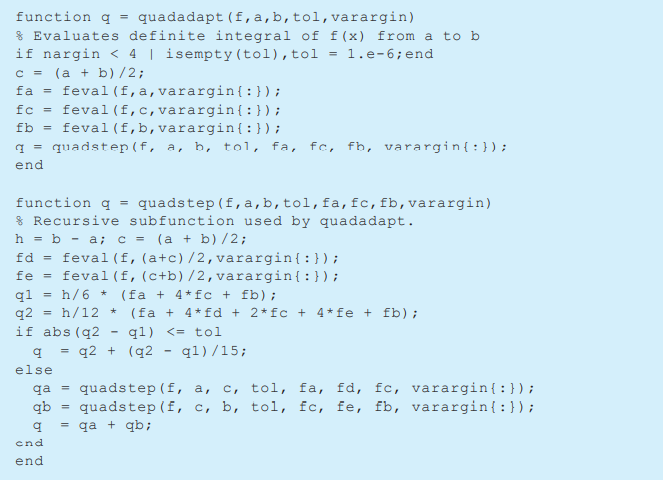
\includegraphics[width=0.75\textwidth]{pic_20_6}
	\caption{\textsf{An M-file to implement an adaptive quadrature algorithm based on an algorithm originally
developed by Cleve Moler (2004).}} \hrule
	\label{pic.20.6}
\end{figure}


\subsection{MATLAB Functions: \small{quad} and \small{quadl}}
MATLAB has two functions, both based on algorithms developed by Gander and Gautschi
(2000), for implementing adaptive quadrature:

\begin{itemize}
	\item \texttt{\textbf{quad.}} This function uses adaptive Simpson quadrature. It may be more efficient for
low accuracies or nonsmooth functions.
	\item \texttt{\textbf{quadl.}} This function uses what is called $Lobatto\, quadrature$. It may be more efficient
for high accuracies and smooth functions.
\end{itemize}

The following function syntax for the quad function is the same for the  \texttt{quadl} 
function:

\begin{verbatim}
    q = quad(fun, a, b, tol, trace, p1, p2, . . .)
\end{verbatim}
where $fun$ is the function to be integrated, $a$ and $b =$ the integration bounds, $tol =$ the
desired absolute error tolerance (default = $10^{−6}$), $trace$ is a variable that when set to a
nonzero value causes additional computational detail to be displayed, and $p1$, $p2$, ...
are parameters that you want to pass to fun. It should be noted that array operators .*, ./
and .\^{} should be used in the definition of $fun$. In addition, pass empty matrices for tol or
$trace$ to use the default values.

\subsection{Adaptive Quadrature}
\textbf{Problem Statement.} Use quad to integrate the following function:

	$$f(x) = \dfrac{1}{(x-q)^{2} +0,01} + \dfrac{1}{(x-r)^{2}+0.04} - s$$\\
between the limits $x = 0$ to $1$. Note that for $q = 0.3$, $r = 0.9$, and $s = 6$, this is the builtin humps function that MATLAB uses to demonstrate some of its numerical capabilities.
The humps function exhibits both flat and steep regions over a relatively short $x$ range.
Hence, it is useful for demonstrating and testing routines like quad and quadl. Note that
the humps function can be integrated analytically between the given limits to yield an exact
integral of 29.85832539549867.\\
\vspace{0.2in}
\textbf{Solution.} First, let's evaluate the integral in the simplest way possible, using the built-in
version of humps along with the default tolerance:
\begin{verbatim}
>> format long
>> quad(@humps,0,1)

ans =
  29.85832612842764
\end{verbatim}
Thus, the solution is correct to seven significant digits.

Next, we can solve the same problem, but using a looser tolerance and passing $q$, $r$, and
$s$ as parameters. First, we can develop an M-file for the function:
\begin{verbatim}
function y = myhumps(x,q,r,s)
y = 1./((x-q).^2 + 0.01) + 1./((x-r).^2+0.04) - s;
\end{verbatim}
Then, we can integrate it with an error tolerance of $10^{−4}$ as in
\begin{verbatim}

>> quad(@myhumps,0,1,le-4,[],0.3,0.9,6)

ans =
  29.85812133214492
\end{verbatim}
Notice that because we used a larger tolerance, the result is now only accurate to five significant digits. However, although it would not be apparent from a single application, fewer
function evaluations were made and, hence, the computation executes faster.


\pagebreak

\subsection{CASE STUDY ROOT-MEAN-SQUARE CURRENT}
\textbf{Background.} Because it results in efficient energy transmission, the current in an AC
circuit is often in the form of a sine wave:

	$$i-i_{peak} \sin(\omega t)$$\\
where $i =$ the current $(A = C/s)$, $i_{peak} =$ the peak current (A), $\omega =$ the angular frequency
(radians/s) and $t$ = time (s). The angular frequency is related to the period $T(s)$ by $\omega = 2\pi/T$.
The power generated is related to the magnitude of the current. Integration can be used
to determine the average current over one cycle:

	$$\bar{i} = \dfrac{1}{T} \int^{T}_{0} i_{peak} \sin (\omega t)dt = \dfrac{i_{peak}}{T} (- \cos(2\pi) + \cos(0)) = 0$$\\
Despite the fact that the average is zero, such a current is capable of generating power.
Therefore, an alternative to the average current must be derived.

To do this, electrical engineers and scientists determine the root mean square current
$i_{rms}$ (A), which is calculated as
\begin{equation}
	\tag{20.31}
	i_{rms} = \sqrt{\dfrac{1}{T} \int^{T}_{0} i^{2}_{peak} \sin^2 (\omega t) dt } = \dfrac{i_{peak}}{\sqrt{2}}
\end{equation}\\
Thus, as the name implies, the rms current is the square root of the mean of the squared current. Because $1/\sqrt{2} = 0.70707$, $i_{rms}$ is equal to about $70\%$ of the peak current for our assumed sinusoidal wave form.

This quantity has meaning because it is directly related to the average power absorbed
by an element in an AC circuit. To understand this, recall that $Joule's \, law$ states that the instantaneous power absorbed by a circuit element is equal to product of the voltage across it
and the current through it:
\begin{equation}
	\tag{20.32}
	P=iV
\end{equation}\\
where $P$ = the power $(W = J/s)$, and $V$ = voltage $(V = J/C)$. For a resistor, $Ohm's \, law states$
that the voltage is directly proportional to the current:
\begin{equation}
	\tag{20.33}
	V=iR
\end{equation}\\
where $R$ = the resistance $(\Omega = V/A = J · s/C^{2})$. Substituting Eq. (20.33) into (20.32) gives
\begin{equation}
	\tag{20.34}
	P=i^{2}R
\end{equation}\\
The average power can be determined by integrating Eq. (20.34) over a period with the result:

	$$\bar{P} = i^{2}_{rms}R$$\\
Thus, the AC circuit generates the equivalent power as a DC circuit with a constant current
of $i_{rms}$.

Now, although the simple sinusoid is widely employed, it is by no means the only
waveform that is used. For some of these forms, such as triangular or square waves, the $i_{rms}$
can be evaluated analytically with closed-form integration. However, some waveforms
must be analyzed with numerical integration methods.

In this case study, we will calculate the root-mean-square current of a non-sinusoidal
wave form. We will use both the Newton-Cotes formulas from Chap. 19 as well as the
approaches described in this section.

\textbf{Solution.} The integral that must be evaluated is
\begin{equation}
	\tag{20.35}
	i^{2}_{rms} = \int^{1/2}_{0} (10e^{-t} \sin 2\pi t)^{2} dt
\end{equation}\\
For comparative purposes, the exact value of this integral to fifteen significant digits is
$15.41260804810169$.

Integral estimates for various applications of the trapezoidal rule and Simpson's 1/3
rule are listed in Table 20.2. Notice that Simpson's rule is more accurate than the trapezoidal
rule. The value for the integral to seven significant digits is obtained using a 128-segment
trapezoidal rule or a 32-segment Simpson's rule.
	
The M-file we developed in Fig. 20.2 can be used to evaluate the integral with
Romberg integration:

\begin{verbatim}
   >> format long
   >> i2=@(t) (10*exp(-t).*sin(2*pi*t)).^2;
   >> [q,ea,iter]=romberg(i2,0,.5)
   q =
     15.41260804288977
   ea =
     1.480058787326946e-008
   iter =
        5
\end{verbatim}

\begin{table}[hbt!]
\caption{\textsf{Values for the integral calculated using Newton-Cotes
formulas. }}
\centering
\begin{tabular}{lccc}
	\hline
	\textbf{Technique} \ \ \ & \ \ \ \textbf{Segments} \ \ \  & \ \ \  \textbf{Integral} \ \ \  & \ \ \  \textbf{$\varepsilon_{t}(\%)$}\\ \hline
	
	Trapezoidal rule & 1 & 0.0 & 100.0000\\
	
	\vspace{0in} & 2 & 15.163266493 & 1.6178\\
	
	\vspace{0in} & 4 & 15.401429095 & 0.0725\\
	
	\vspace{0in} & 8 & 15.411958360 &  4.22 × $10^{-3}$\\
	
	\vspace{0in} & 16 & 15.412568151 & 2.59 × $10^{-4}$\\
	
	\vspace{0in} & 32 &  15.412605565 & 1.61 × $10^{-5}$\\
	
	\vspace{0in} & 64 &  15.412607893 &  1.01 × $10^{-6}$\\
	
	\vspace{0in} & 128 & 15.412608038 & 6.28 × $10^{-8}$\\ \hline
	
	Simpson's 1/3 rule & 2 & 20.217688657 & 31.1763\\
	
	\vspace{0in} & 4 & 15.480816629 &  0.4426\\
	
	\vspace{0in} & 8 & 15.415468115 & 0.0186\\
	
	\vspace{0in} & 16 & 15.412771415 & 1.06 × $10^{-3}$\\
	
	\vspace{0in} & 32 & 15.412618037 & 6.48 × $10^{-5}$\\ \hline
\end{tabular}
\end{table}
Thus, with the default stopping criterion of $es = 1 × 10^{−6}$
, we obtain a result that is correct
to over nine significant figures in five iterations. We can obtain an even better result if we
impose a more stringent stopping criterion:
\begin{verbatim}
   >> [q,ea,iter]=romberg(i2,0,.5,1e-15)
   q =
     15.41260804810169
   ea =
        0
   iter =
        7
\end{verbatim}

Gauss quadrature can also be used to make the same estimate. First, a change in
variable is performed by applying Eqs. (20.22) and (20.23) to yield

	$$t= \dfrac{1}{4} + \dfrac{1}{4}t_{d} \; \; \; \; \; \; \; \; \; \; \; \; dt=\dfrac{1}{4} dt_{d} $$\\
These relationships can be substituted into Eq. (20.35) to yield

\begin{equation}
	\tag{20.36}
	i^{2}_{rms} = \int^{1}_{-1} [10e^{-(0.25+025t_{d})} \sin 2\pi (0.25+0.25t_{d})]^{2} 0.25 dt
\end{equation}\\
For the two-point Gauss-Legendre formula, this function is evaluated at $t_{d} = −1/\sqrt{3}$ and $1/\sqrt{3}$ , with the results being $7.684096$ and $4.313728$, respectively. These values can be
substituted into Eq. (20.17) to yield an integral estimate of $11.99782$, which represents an
error of $\varepsilon_{t} = 22.1\%$.

The three-point formula is (Table 20.1)

$$I = 0.5555556(1.237449) + 0.8888889(15.16327) + 0.5555556(2.684915) = 15.65755$$\\
which has $\varepsilon_{t} = 1.6\%$. The results of using the higher-point formulas are summarized in
Table 20.3.

Finally, the integral can be evaluated with the built-in MATLAB function quad and quadl:
\begin{verbatim}
   >> irms2=quad(i2,0,.5)
   irms2 =
     15.41260804934509
\end{verbatim}

\begin{table}[hbt!]
\caption{\textsf{Results of using various-point Gauss quadrature
formulas to approximate the integral.  }}
\centering
\begin{tabular}{ccc}
	\hline
	\textbf{Points} \ \ \ \ \ & \ \ \ \ \ \textbf{Estimate} \ \ \ \ \  & \ \ \ \ \  \textbf{$\varepsilon_{t} (\%)$}\\ \hline
	
	2 & 11.9978243 & 22.1\\

	3 & 15.6575502 & 1.59\\

	4 & 15.4058023 & 4.42 × $10^{-2}$\\
	
	5 & 15.4126391 & 2.01 × $10^{-4}$\\
	
	6 & 15.4126109 & 1.82 × $10^{-5}$\\ \hline
\end{tabular}
\end{table}

\begin{verbatim}
   >> irms2=quadl(i2,0,.5)
   
   irms2 =
     15.41260804809967
\end{verbatim}
Both these results are very accurate, with quadl being a little better.

We can now compute the $i_{rms}$ by merely taking the square root of the integral. For example, using the result computed with quadl, we get

\begin{verbatim}
   >> irms=sqrt(irms2)
   
   irms =
      3.92588945948554
\end{verbatim}
This result could then be employed to guide other aspects of the design and operation of the
circuit such as power dissipation computations.

As we did for the simple sinusoid in Eq. (20.31), an interesting calculation involves
comparing this result with the peak current. Recognizing that this is an optimization problem, we can readily employ the fminbnd function to determine this value. Because we are
looking for a maximum, we evaluate the negative of the function:

\begin{verbatim}
   >> [tmax,imax]=fminbnd(@(t) -10*exp(-t).*sin(2*pi*t),0,.5)
   tmax =
     0.22487940319321
   imax =
     -7.88685387393258
\end{verbatim}
A maximum current of $7.88685$ A occurs at $t = 0.2249$ s. Hence, for this chaptericular wave
form, the root-mean-square value is about $49.8\%$ of the maximum.
\\
\section*{PROBLEMS} \hrule

\begin{multicols}{2}
\textbf{20.1} Use Romberg integration to evaluate

	$$I = \int^{2}_{1} \left( x+\dfrac{1}{x} \right)^{2} dx$$\\
to an accuracy of $\varepsilon_{s} = 0.5\%$. Your results should be presented
in the format of Fig. 20.1. Use the analytical solution of the
integral to determine the percent relative error of the result obtained with Romberg integration. Check that $\varepsilon_{t}$ is less than $\varepsilon_{s}$.

\textbf{20.2} Evaluate the following integral \textbf{(a)} analytically,
\textbf{(b)} Romberg integration $(\varepsilon_{s} = 0.5\%)$, \textbf{(c)}the three-point Gauss quadrature formula, and \textbf{(d)} MATLAB quad function:

	$$I= \int^{8}_{0} -0.055x^{4} + 0.86x^{3} - 4.2x^{2} + 6.3x + 2dx$$
	
\textbf{20.3} Evaluate the following integral with \textbf{(a)} Romberg integration $(\varepsilon_{s} = 0.5\%)$, \textbf{(b)} the two-point Gauss quadrature
formula, and \textbf{(c)} MATLAB quad and quadl functions:

	$$I = \int^{3}_{0} xe^{2x} dx$$
	
\textbf{20.4} There is no closed form solution for the error function

	$$erf(a) = \dfrac{2}{\sqrt{\pi}} \int^{a}_{0} e^{-x^{2}} dx$$\\
Use the \textbf{(a)} two-point and \textbf{(b)} three-point Gauss-Legendre
formulas to estimate erf(1.5). Determine the percent relative
error for each case based on the true value, which can be determined with MATLAB's built-in function erf.

\textbf{20.5} The force on a sailboat mast can be represented by the
following function:

	$$F= \int^{H}_{0} 200 \left(\dfrac{z}{5+z} \right) e^(-2z/H) dz $$\\
where $z$ = the elevation above the deck and $H$ = the height
of the mast. Compute $F$ for the case where $H = 30$ using
\textbf{(a)} Romberg integration to a tolerance of $\varepsilon_{s} = 0.5\%$, \textbf{(b)} the
two-point Gauss-Legendre formula, and \textbf{(c)} the MATLAB
quad function.

\textbf{20.6} The root-mean-square current can be computed as

	$$I_{RMS} = \sqrt{\dfrac{1}{T} \int^{T}_{0} i^{2} (t) dt}$$\\
For $T = 1$, suppose that $i(t)$ is defined as

	$$ i(t) = 8e^{-t/T} \sin \left( 2\pi \dfrac{t}{T} \right) \; \; \; for \; \; \; 0 \leq t \leq T/2$$
	
	$$i(t) = 0 \; \; \; \; \; for \; \; \; T/2 \leq t \leq T$$\\
Evaluate the $I_{RMS}$ using \textbf{(a)} Romberg integration to a tolerance of $0.1\% $, \textbf{(b)} the two- and three-point Gauss-Legendre
formulas, and \textbf{(c)} the MATLAB quad function.

\textbf{20.7} The heat required, $\Delta H$(cal), to induce a temperature change, $\Delta T(^{\circ} C)$, of a material can be computed as

	$$\Delta H = mC_{p} (T) \Delta T$$\\
where $m$ = mass (g), and $C_{p}(T)$  heat capacity $[cal/(g .^{\circ}C)]$.
The heat capacity increases with temperature, $T (^{\circ}C)$, 
according to

	$$C_{p} (T) = 0.132 + 1.56 × 10^{-4} T + 2.64 × 10^{-7} T^2$$\\
Write a script that uses the quad function to generate a plot
of $\Delta H$ versus $\Delta T$ for cases where $m$ = 1kg, the starting
temperature is -100$^{\circ}$ C and $\Delta T$ ranges from 0 to 300 $^{\circ}$ C.

\textbf{20.8} The amount of mass transported via a pipe over a period of time can be computed as

	$$M=\int^{t_{2}}_{t_{1}} Q(t)c(t) dt$$\\
where $M$ = mass (mg), $t_{1}$ = the initial time (min), $t_{2}$ = the
final time (min), $Q(t)$ = flow rate $(m^{3}
/min)$, and $c(t)$ =
concentration $(mg/m^{3})$. The following functional representations define the temporal variations in flow and
concentration:

	$$Q(t) = 9 + 5 \cos^{2}(0.4t) $$
	
	$$c(t) = 5e^{-0.5t} + 2e^{0.15t}$$\\
Determine the mass transported between $t_{1} = 2$ and
$t_{2} = 8$ min with \textbf{(a)} Romberg integration to a tolerance of
$0.1\%$ and \textbf{(b)} the MATLAB quad function.

\textbf{20.9} Evaluate the double integral

	$$\int^{2}_{-2} \int^{4}_{0} (x^{2} - 3y^{2} + xy^{3}) dx dy$$\\
\textbf{(a)} analytically and \textbf{(b)} using the MATLAB dblquad 
function. Use help to understand how to implement the
function.

\textbf{20.10} Compute work as described in Sec. 19.9, but use the
following equations for $F(x)$ and $\theta(x)$:

	$$F(x) = 1.6x - 0.045x^{2}$$
	
	$$\theta(x) = -0.00055x^{3} + 0.0123x^{2} + 0.13x $$\\
The force is in newtons and the angle is in radians. Perform
the integration from $x$ = 0 to 30 m.

\textbf{20.12} Compute the power absorbed by an element in a circuit as described in Sec. 20.5, but for a simple sinusoidal
current $i = \sin (2\pi t/T)$ where $T$ = 1 s. \\
\textbf{(a)} Assume that Ohm's law holds and $R = 5 \\Omega$.\\
\textbf{(b)} Assume that Ohm's law does not hold and that voltage
and current are related by the following nonlinear relationship: $V = (5i - 1.25i^{3})$.

\textbf{20.13} Suppose that the current through a resistor is described by the function

	$$i(t) = (60 - t)^{2} + (60 - t) \sin (\sqrt{t})$$\\
and the resistance is a function of the current:

	$$R = 10i + 2i^{2/3}$$\\
Compute the average voltage over $t$ = 0 to 60 using the
composite Simpson's 1/3 rule.

\end{multicols}

\pagebreak


\begin{figure}[hbt!]
	\centering
	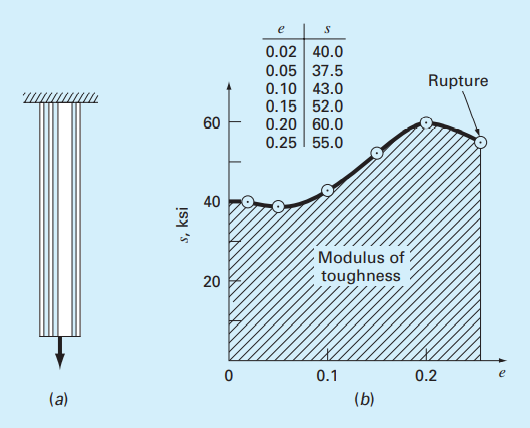
\includegraphics[width=0.55\textwidth]{pic_20_7}
	\caption{\textsf{(a) A rod under axial loading and (b) the resulting stress-strain curve, where
stress is in kips per square inch (103 lb/in2
), and strain is dimensionless.}} \hrule
	\label{pic.20.7}
\end{figure}


\begin{multicols}{2}
\textbf{20.14} If a capacitor initially holds no charge, the voltage
across it as a function of time can be computed as 

	$$V(t) = \dfrac{1}{C} \int^{t}_{0} i(t) dt$$\\
Use MATLAB to fit these data with a fifth-order polynomial.
Then, use a numerical integration function along with a value
of $C = 10^{−5}$ farad to generate a plot of voltage versus time.\\
\begin{tabular}{ccccc}
	\hline

\textbf{$t$,s} & 0 & 0.2 & 0.4 & 0.6\\

\textbf{$i, 10^{-3}$A} & 0.2 &  0.3683 &  0.3819 &  0.2282\\

\vspace{0in}\\

\textbf{$t$, s} & 0.8 & 1 & 1.2 & \vspace{0in}\\

\textbf{$i, 10^{-3}$A} & 0.0486 & 0.0082 & 0.1441 & \vspace{0in}\\ \hline
\end{tabular}


\textbf{20.15} The work done on an object is equal to the force times
the distance moved in the direction of the force. The velocity of an object in the direction of a force is given by\\
\begin{tabular}{ll}
$v =4t$ & $0 \leq t \leq 5$\\
$v = 20 + (5-t)^{2}$  &  $5 \leq t \leq 15$
\end{tabular}\\
where $v$ is in m/s. Determine the work if a constant force of
200 N is applied for all $t$.

\textbf{20.16} A rod subject to an axial load (Fig. P20.16a) will be
deformed, as shown in the stress-strain curve in Fig. P20.16b. The area under the curve from zero stress out to the point of
rupture is called the $modulus\, of\, toughness$ of the material. It
provides a measure of the energy per unit volume required to
cause the material to rupture. As such, it is representative of
the material's ability to withstand an impact load. Use numerical integration to compute the modulus of toughness for
the stress-strain curve seen in Fig. P20.16b

\textbf{20.17} If the velocity distribution of a fluid flowing through
a pipe is known (Fig. P20.17), the flow rate $Q$ (i.e., the volume of water passing through the pipe per unit time) can be
computed by $Q = \int v dA$, where $v$ is the velocity, and A is
the pipe's cross-sectional area. (To grasp the meaning of this
relationship physically, recall the close connection between
summation and integration.) For a circular pipe, $A = \pi r^{2}$ and $dA = 2 \pi r dr$. Therefore,

	$$Q = \int^{r}_{0} v(2 \pi r) dr$$
	



\end{multicols}

\begin{figure}[hbt!]
	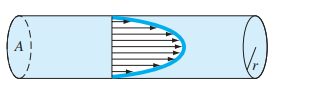
\includegraphics[width=0.35\textwidth]{pic_20_8}
	\caption{} \hrule
	\label{pic.20.8}
\end{figure}

\begin{multicols}{2}
where r is the radial distance measured outward from the
center of the pipe. If the velocity distribution is given by

	$$v = 2 \left( 1- \dfrac{r}{r_{0}} \right)^{1/6}$$\\
where $r_(0)$ is the total radius (in this case, 3 cm), compute $Q$
using the composite trapezoidal rule. Discuss the results.

\textbf{20.18} Using the following data, calculate the work done by
stretching a spring that has a spring constant of $k$ = 300 N/m
to $x$ = 0.35 m. To do this, first fit the data with a polynomial
and then integrate the polynomial numerically to compute
the work:\\
\vspace{0.3in}
\begin{tabular}{lcccc}
\hline
\textbf{$F,10^{3} \cdot N$} & 0 & 0.01 & 0.028 & 0.046\\

\textbf{$x, m$} & 0 & 0.05 & 0.10 & 0.15\\

\vspace{0in}\\

\textbf{$F, 10^{3} \cdot N$} & 0.063 & 0.082 & 0.11 & 0.13\\

\textbf{$x, m$} & 0.20 & 0.25 & 0.30 & 0.35\\ \hline
\end{tabular}

\textbf{20.19} Evaluate the vertical distance traveled by a rocket if
the vertical velocity is given by

\begin{tabular}{ll}
$v=11t^{2} - 5t$ & $0 \leq t \leq 10$\\
$v=1100 - 5t$ & $10 \leq t \leq 20$\\
$v=50t + 2(t-20)^{2}$ & $20 \leq t \leq 30$\\
\end{tabular}

\textbf{20.20} The upward velocity of a rocket can be computed by
the following formula:

	$$v = u ln \left( \dfrac{m_{0}}{m_{0} - qt} \right) - gt$$\\
where $v$ = upward velocity, $u$ = velocity at which fuel is expelled relative to the rocket, $m_{0}$ = initial mass of the rocket
at time $t = 0$, $q$ = fuel consumption rate, and $g$ = downward
acceleration of gravity (assumed constant = $9.81 m/s^{2}$
). If $u = 1850 m/s$, $m_{0}$ = 160,000 kg, and $q$ = 2500 kg/s, determine
how high the rocket will fly in 30 s.

\textbf{20.21} The normal distribution is defined as

	$$f(x) = \dfrac{1}{\sqrt{2 \pi}} e^{-x2/2}$$\\
\textbf{(a)} Use MATLAB to integrate this function from $x = −1$ to
1 and from −2 to 2.\\
\textbf{(b)} Use MATLAB to determine the inflection points of this
function.

\textbf{20.22} Use Romberg integration to evaluate

	$$\int^{2}_{0} \dfrac{e^{x} \sin x}{1+x^{2}} dx$$\\
to an accuracy of $\varepsilon_{s} = 0.5\%$ Your results should be presented in the form of Fig. 20.1.

\textbf{20.23} Recall that the velocity of the free-falling bungee
jumper can be computed analytically as [(Eq. 1.9)]:

	$$v(t) = \sqrt{\dfrac{gm}{c_{d}}} tanh \left( \sqrt{\dfrac{gc_{d}}{m}} t \right)$$\\
where $v(t)$ = velocity (m/s), $t$ = time (s), g = 9.81 m/s2
, 
$m$ = mass (kg), $c_{d}$ = drag coefficient (kg/m). \\
\textbf{(a)} Use Romberg integration to compute how far the jumper
travels during the first 8 seconds of free fall given $m$ =
80 kg and $c_{d}$ = 0.2 kg/m. Compute the answer to $\varepsilon_{s} = 1\%$.
\textbf{(b)} Perform the same computation with quad.

\textbf{20.24} Prove that Eq. (20.30) is equivalent to Boole's rule.

\textbf{20.25} As specified in the following table, the earth's density
varies as a function of the distance from its center ($r$ = 0):\\
\begin{tabular}{lccccccc}
	\hline

\scriptsize{\textbf{$r, km$}} & \scriptsize{0} & \scriptsize{1100} & \scriptsize{1500} & \scriptsize{2450} & \scriptsize{3400} & \scriptsize{3630} & \scriptsize{4500}\\

\scriptsize{\textbf{$\rho, g/cm^{3}$}} & \scriptsize{13} & \scriptsize{12.4} & \scriptsize{12} & \scriptsize{11.2} & \scriptsize{9.7} & \scriptsize{5.7} & \scriptsize{5.2}\\

\vspace{0in}\\

\scriptsize{\textbf{$r,km$}} & \scriptsize{5380} & \scriptsize{6060} & \scriptsize{6280} & \scriptsize{6380} & \vspace{0in} & \vspace{0in} & \vspace{0in}\\

\scriptsize{\textbf{$\rho, g/cm^{3}$}} & \scriptsize{4.7} & \scriptsize{3.6} & \scriptsize{3.4} & \scriptsize{3} & \vspace{0in} & \vspace{0in} & \vspace{0in}\\ \hline

\end{tabular}\\
Develop a script to fit these data with interp1 using the
pchip option. Generate a plot showing the resulting fit
along with the data points. Then use one of MATLAB's integration functions to estimate the earth's mass (in metric
tonnes) by integrating the output of the interp1 function.

\textbf{20.26} Develop an M-file function to implement Romberg integration based on Fig. 20.2. Test the function by using it to
determine the integral of the polynomial from Example 20.1.
Then use it to solve Prob. 20.1.

\textbf{20.27} Develop an M-file function to implement adaptive
quadrature based on Fig. 20.6. Test the function by using it to
determine the integral of the polynomial from Example 20.1.
Then use it to solve Prob. 20.20.




\end{multicols}



\end{document}